% \chapter{Drawings - Robot end effector}\label{cha:endeffector}
% \begin{figure}[h]
%     \centering
%     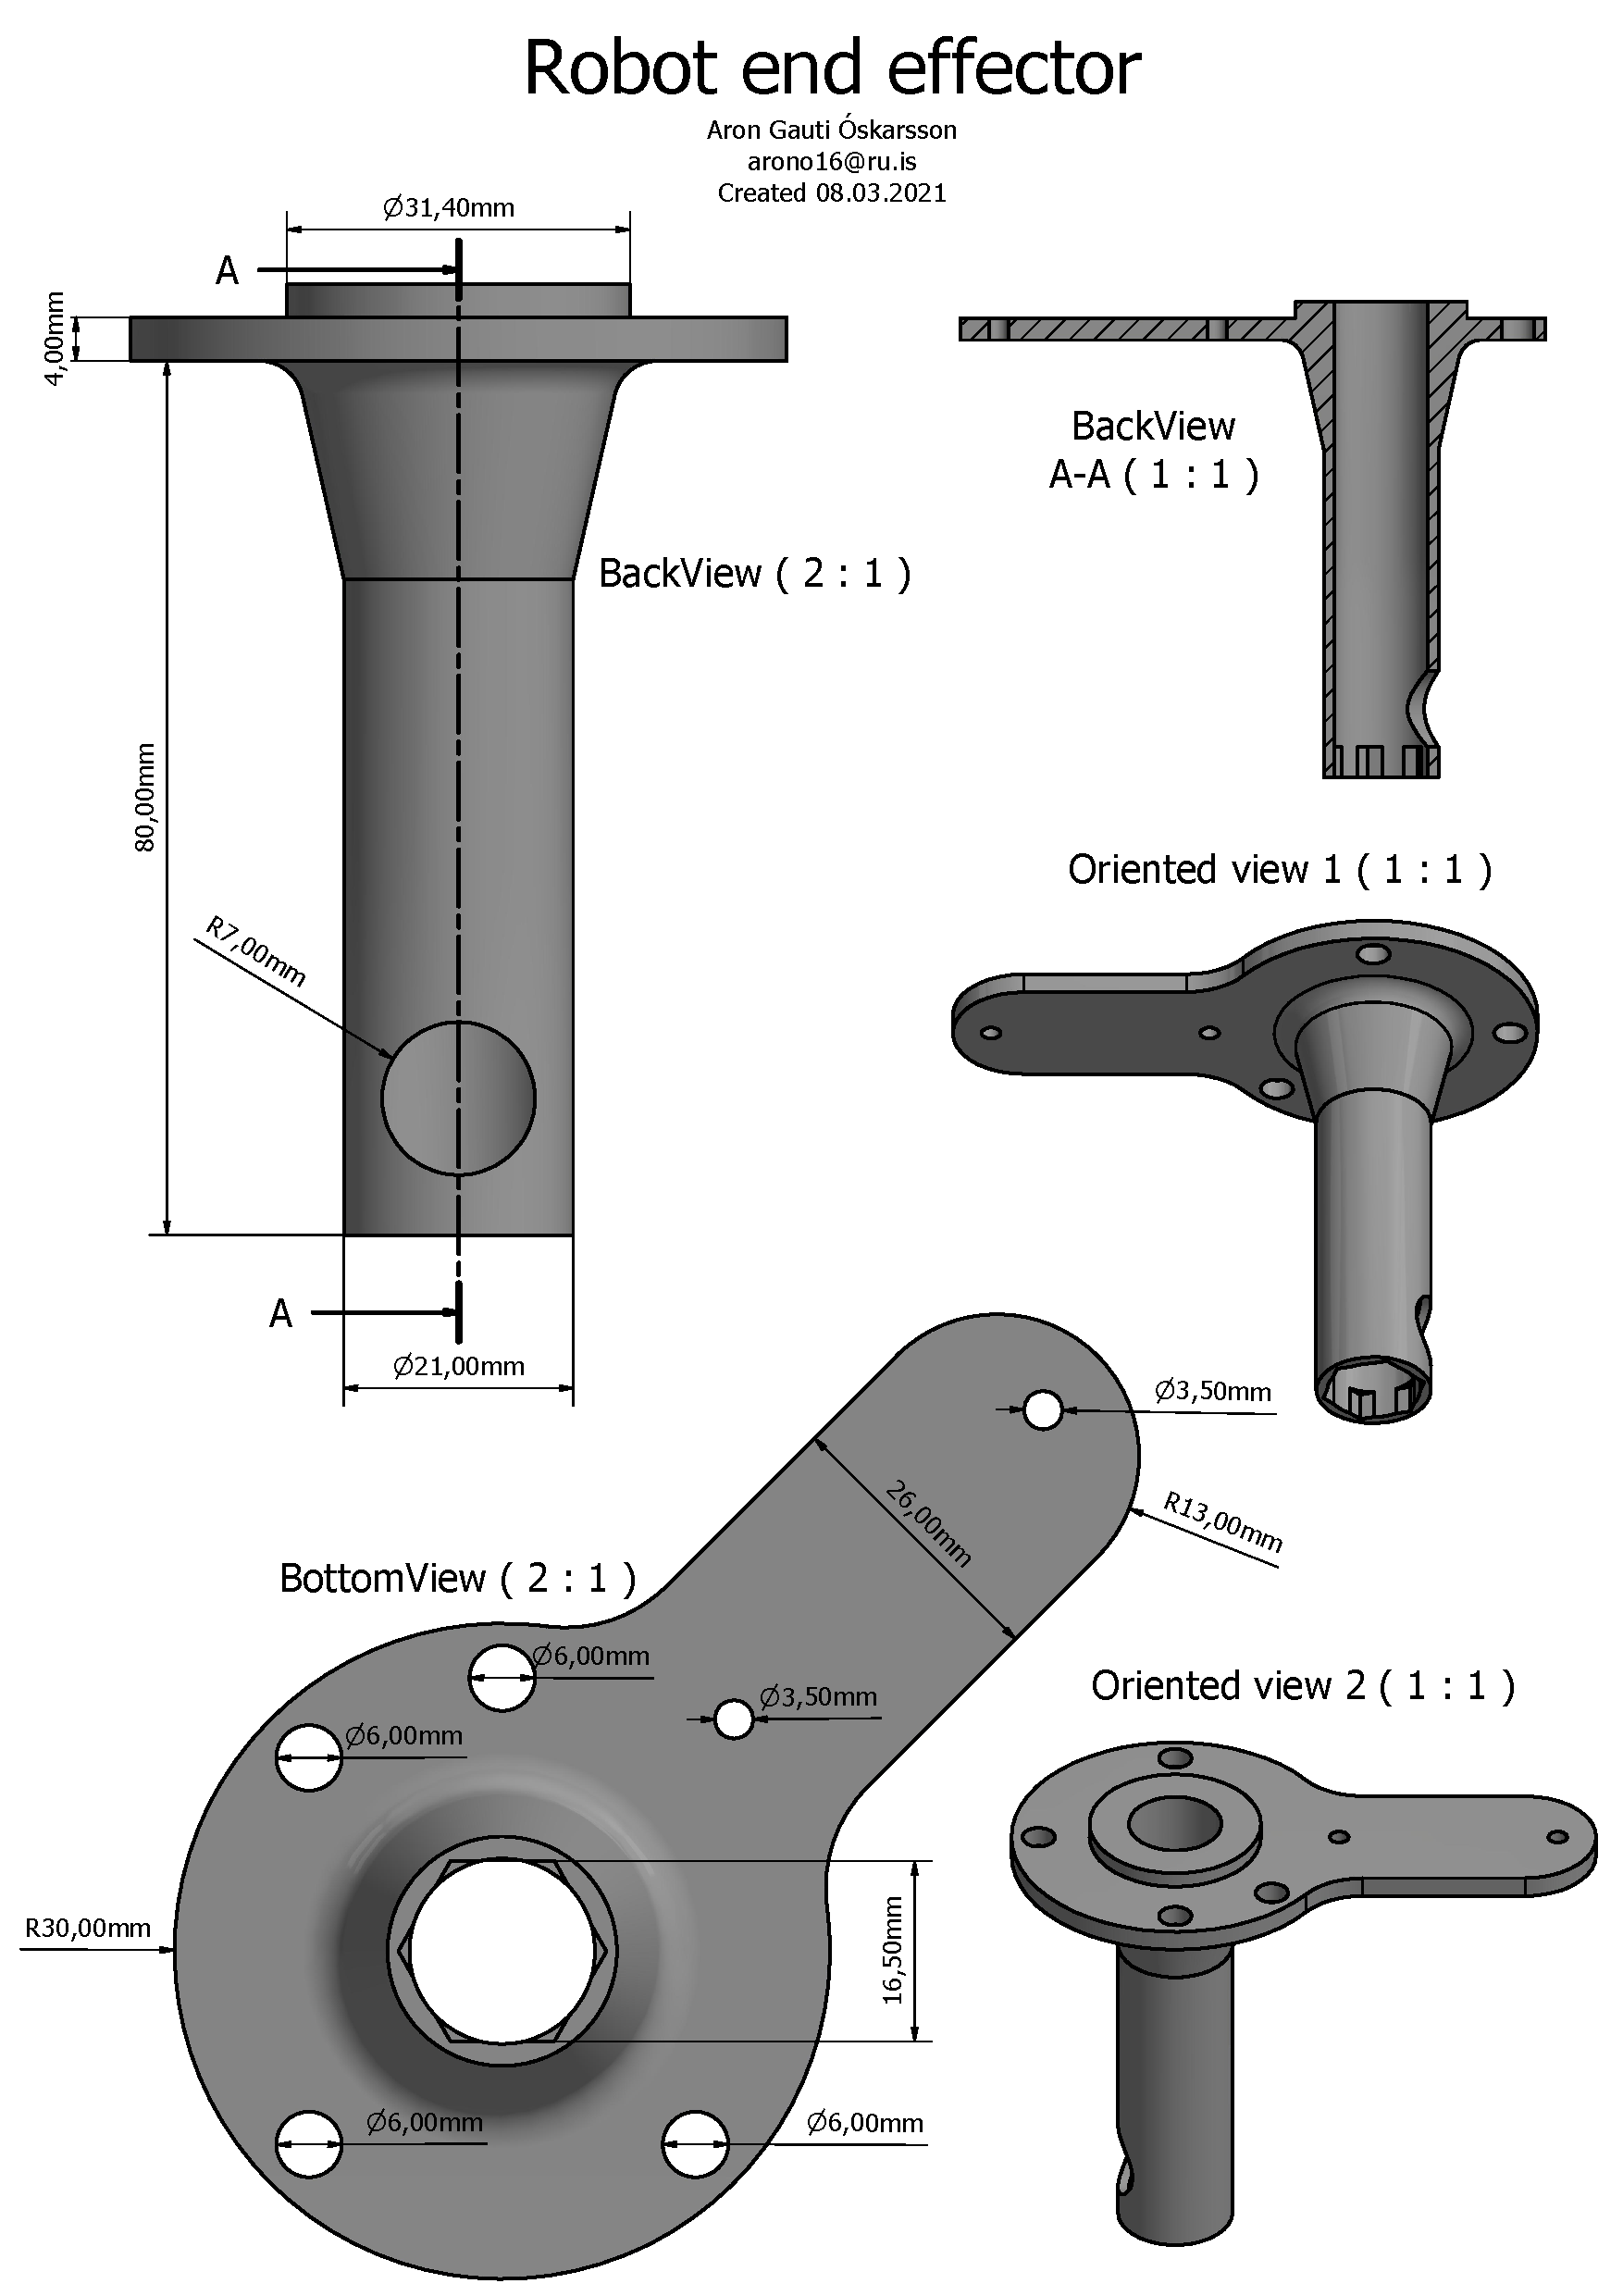
\includegraphics[width=0.7\textwidth]{graphics/model_panda_vacuumnewportrait.pdf}
%     \caption{Robot end effector}
%     \label{fig:my_label}
% \end{figure}
%Hægt að vera með tvær týpur sýnist þessi fyrir neðan betri

\definecolor{gray}{rgb}{0.4,0.4,0.4}
\definecolor{darkblue}{rgb}{0.0,0.0,0.6}
\definecolor{cyan}{rgb}{0.0,0.6,0.6}

\lstset{
  basicstyle=\ttfamily,
  columns=fullflexible,
  showstringspaces=false,
  commentstyle=\color{gray}\upshape
}

\lstdefinelanguage{XML}
{
  morestring=[b]",
  morestring=[s]{>}{<},
  morecomment=[s]{<?}{?>},
  stringstyle=\color{black},
  identifierstyle=\color{darkblue},
  keywordstyle=\color{cyan},
  morekeywords={xmlns,version,type}% list your attributes here
}
\appendix

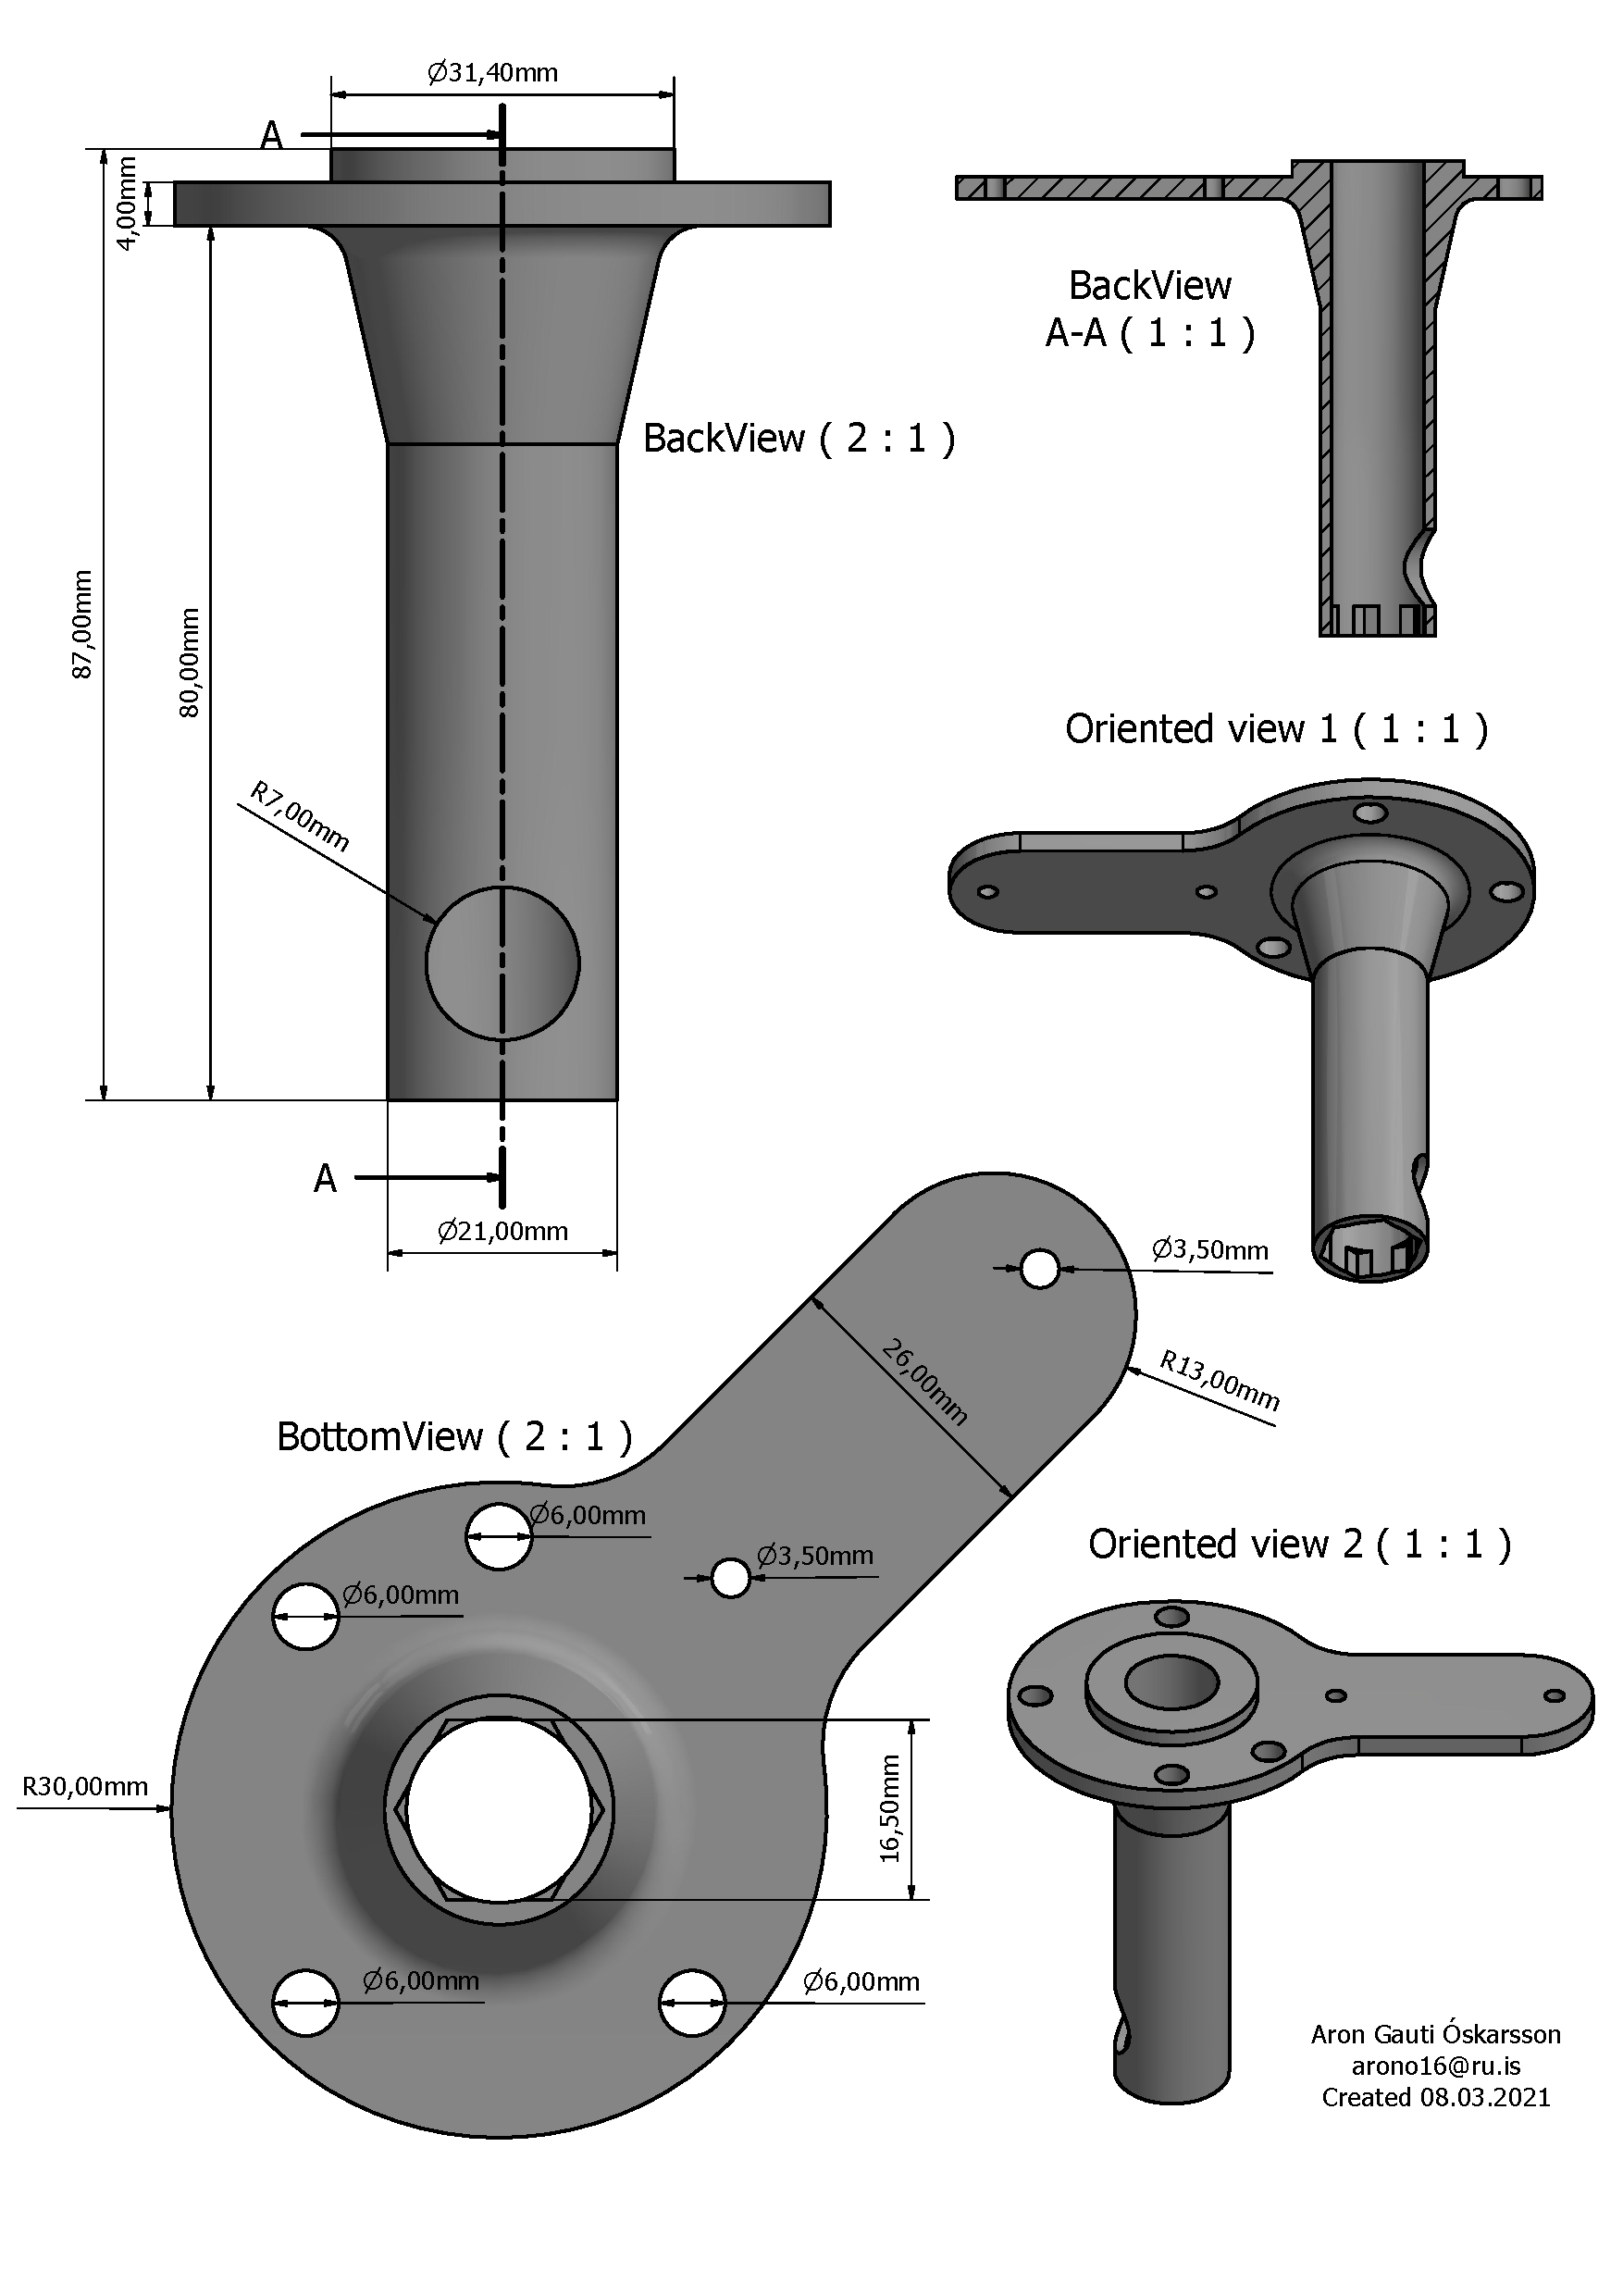
\includepdf[scale=0.7,pages=1,pagecommand=\chapter{Drawings - Robot end effector}\label{cha:endeffector}, offset=0 -4cm]{graphics/suctionDrawing.pdf}

\chapter{Code}
\section{pick-and-place.py}\label{sec:pickandplace}
%\lstinputlisting[language=Python]{code/pick_and_place.py}
\pagebreak
\section{find-pickpoint.py}\label{sec:findpickpoint}
%\lstinputlisting[language=Python]{code/find_pick_point.py}
\pagebreak
\section{difference.py}\label{sec:difference}
%\lstinputlisting[language=Python]{code/difference.py}
\pagebreak
\section{panda-bringup.launch}\label{sec:pandabringup}
\lstinputlisting[language=XML]{code/panda_bringup.launch}